\documentclass[conference]{IEEEtran}
\usepackage{babel}
\usepackage[utf8]{vietnam}
\usepackage{mathtools}
\usepackage{graphicx}
\usepackage{graphics}
\usepackage{epstopdf}
\usepackage{amsfonts}
\usepackage{siunitx}
\providecommand{\keywords}[1]
{
	\small	
	\textbf{\textit{Keywords---}} #1
}
\begin{document}
	\title{Thiết kế phần cứng cho biến đổi 2D-DCT 64 điểm}
	\author{Nhóm 18: Trương Bá Mạnh, Chu Tiến Thịnh, Phạm Văn Nguyện}
	\maketitle
	\begin{abstract}
		Đề tài này đưa ra phương pháp thiết kế phần cứng cho biến đổi 2D-DCT 64 điểm, sử dụng các bộ cộng và bộ nhân song song, thiết kế bằng ngôn ngữ Verilog và mô phỏng trên ModelSim.
	\end{abstract}
	\keywords{DCT, Verilog}
	\section{Giới thiệu chung}
	Discrete Cosine Transform (DCT) là phép biến đổi biểu diễn một tập hữu hạn điểm dưới dạng các hàm $\cos$ tại các tần số khác nhau. Biến đổi DCT có nhiều loại, trong đó phổ biến nhất là 2D-DCT. DCT chủ yếu được ứng dụng trong nén ảnh và video. Nó loại bỏ dư thừa về mặt không gian bằng cách biến đổi miền không gian sang miền tần số \cite{art1}.\\
	Trong những năm qua, đã nhiều công trình nghiên cứu về DCT. Phép biến đổi 2D-DCT trực tiếp \cite{art2} cho hiệu quả thấp về mặt tính toán song song, trong khi phép biến đổi theo từng hàng và cột \cite{art3}\cite{art4} cho tốc độ nhanh hơn. Nhiều sự thay đổi về thuật toán được đề xuất nhắm giảm độ phức tạp của thuật toán \cite{art5}\cite{art6}\cite{art7}. Một thuật toán song song, tuyến tính sử dụng pipeline cho phép biến đổi 2D-DCT và lượng tử hóa được đề xuất trong \cite{art8}\cite{art9}. Kiến trúc được đề xuất trong hai bài báo này giảm thiểu những hạn chế của các phương pháp được trích dẫn trước đó. Phương pháp này sử dụng các đầu vào song song để giảm thời gian nạp dữ liệu. Đề tài này chủ yếu dựa trên \cite{book1}. 
	\section{Thuật toán DCT}
	Phép biến đổi 2D-DCT cho khối 8 x 8 được định nghĩa là:
	\begin{align*}
	DCT(u,v) = \frac{1}{4}c(u)c(v)\sum_{x = 0}^{7}\sum_{y = 0}^{7}f(x, y)&[\cos\frac{(2x + 1)u\pi}{16}]\\
	&[\cos\frac{(2y + 1)v\pi}{16}]
	\end{align*}
	Trong đó $f(x, y)$ là cường độ điểm ảnh và:
	\[
	c(u) = c(v) = \begin{cases*}
	\frac{1}{\sqrt{2}} \quad \text{khi u = v = 0}\\
	1 \quad \text{còn lại}
	\end{cases*}
	\]
	Ta có thể biểu diễn dưới dạng ma trận:
	\begin{equation*}
	DCT = C X C^T
	\end{equation*}
	Trong đó $X$ là ma trận đầu vào, $C$ là các hệ số $\cos$ và $C^T$ là ma trận chuyển vị của $C$, các hằng số $\frac{1}{2}c(u)$ và $\frac{1}{2}c(v)$ được nhân với ma trận $C$ và $C^T$.\\
	Ta biểu diễn một cách rõ ràng hơn như sau:
	\[DCT = 
	\begin{bmatrix}
	c_{00} &\dots &c_{07}\\
	\vdots &\ddots &\vdots\\
	c_{70} &\dots &c_{77}
	\end{bmatrix}
	\begin{bmatrix}
	x_{00} &\dots &x_{07}\\
	\vdots &\ddots &\vdots\\
	x_{70} &\dots &x_{77}
	\end{bmatrix}
	\begin{bmatrix}
	c_{00} &\dots &c_{70}\\
	\vdots &\ddots &\vdots\\
	c_{07} &\dots &c_{77}
	\end{bmatrix}		
	\]
	\[=
	\begin{bmatrix}
	p_{00} &\dots &p_{07}\\
	\vdots &\ddots &\vdots\\
	p_{70} &\dots &p_{77}
	\end{bmatrix}
	\begin{bmatrix}
	c_{00} &\dots &c_{70}\\
	\vdots &\ddots &\vdots\\
	c_{07} &\dots &c_{77}
	\end{bmatrix}
	\]
	\[=
	\begin{bmatrix}
	\sum_{i=0}^{7}p_{0i}c_{0i} &\dots &\sum_{i=0}^{7}p_{0i}c_{7i}\\
	\vdots &\ddots &\vdots\\
	\sum_{i=0}^{7}p_{7i}c_{0i} &\dots &\sum_{i=0}^{7}p_{7i}c_{7i}
	\end{bmatrix}
	\]
	\section{Architecture}
	\subsection{Bộ cộng song song}
	Kiến trúc của bộ cộng song song được thể hiện trong Hình \ref{adder}.\\
	\begin{figure}[h]
		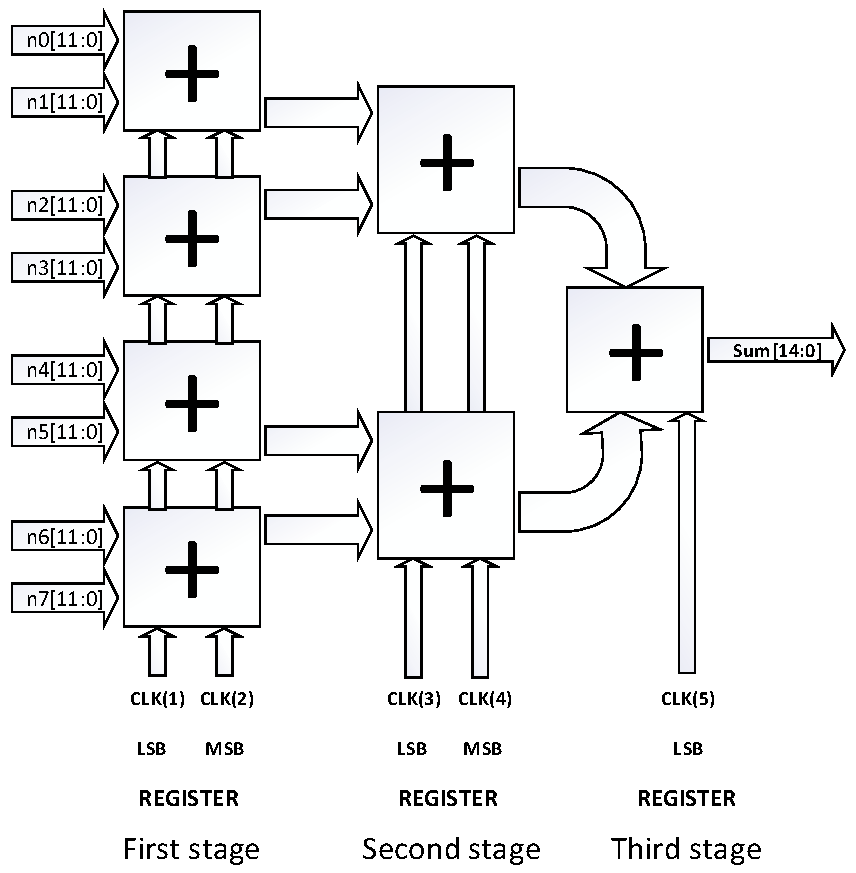
\includegraphics[width=\linewidth]{Figures/adder.pdf}
		\caption{Kiến trúc bộ cộng song song} 
		\label{adder}
	\end{figure}
	Quá trình cộng được chia thành ba giai đoạn pipeline. Ở giai đoạn đầu tiên, ta có 4 số 12 bits và 2 bộ cộng để cộng 8 số, chúng hoạt động đồng thời, do đó làm tăng tốc độ xử lý. Chúng có các thanh ghi pipeline, xung clock đầu vào được đánh số (1), (2), ... tương ứng với các thanh ghi pipeline. Ta sẽ cộng LSBs ở xung clock đầu tiên và MSBs ở xung tiếp theo cùng với bit nhớ từ LSB. Ở chặng thứ hai, ta cộng 4 đầu ra ở giai đoạn thứ nhất, mỗi đầu ra 13 bits. Hai số của hai bộ cộng đàu vào được dùng ở giai đoạn này. LSBs và MSBs được cộng khi xuất hiện xung clock. Ở giai đoạn thứ ba, khi xung clock xuất hiện, ta sẽ cộng LSBs của 2 đầu vào 14 bits. Tiếp theo, MSBs được cộng cùng với bit nhớ từ LSBs và cho kết quả 15 bits.
	\subsection{Bộ nhân song song}
	Quá trình nhân song song gồm tám giai đoạn pipeline,  được thể hiện trong Hình \ref{mul}.\\
	\begin{figure}[h]
		\includegraphics[width=\linewidth]{Figures/mul.pdf}
		\caption{Kiến trúc bộ nhân song song} 
		\label{mul}
	\end{figure}
	Phép nhân được thực hiện chủ yếu trên thành phần độ lớn của hai số, vì vậy chúng ta cần tách riêng phần dấu và độ lớn bằng cách sử dụng cổng or. Ở giai đoạn đầu tiên, ta cộng 4 cặp số và được 4 kết quả tương ứng là S11, S12, S13, S14. Chúng ta cộng P1 và P2 sau khi dịch trái P2 1 bit. Tương tự cho các cặp P3/P4, P5/P6, P7/P8 ở chặng đầu tiên, chúng được thực hiện đồng thời. Xung clock được đánh số (1), (2), ... ứng với các thanh ghi pipeline ở các chặng khác nhau. Các tích P1 tới P8 đạt được bằng phép $\text{and}$ bội số với số nhân ứng với các bit của số nhân.
	\subsection{Kiến trúc DCT}
	Kiến trúc DCT được thể hiện trong Hình \ref{sys}.
	\begin{figure}[h]
		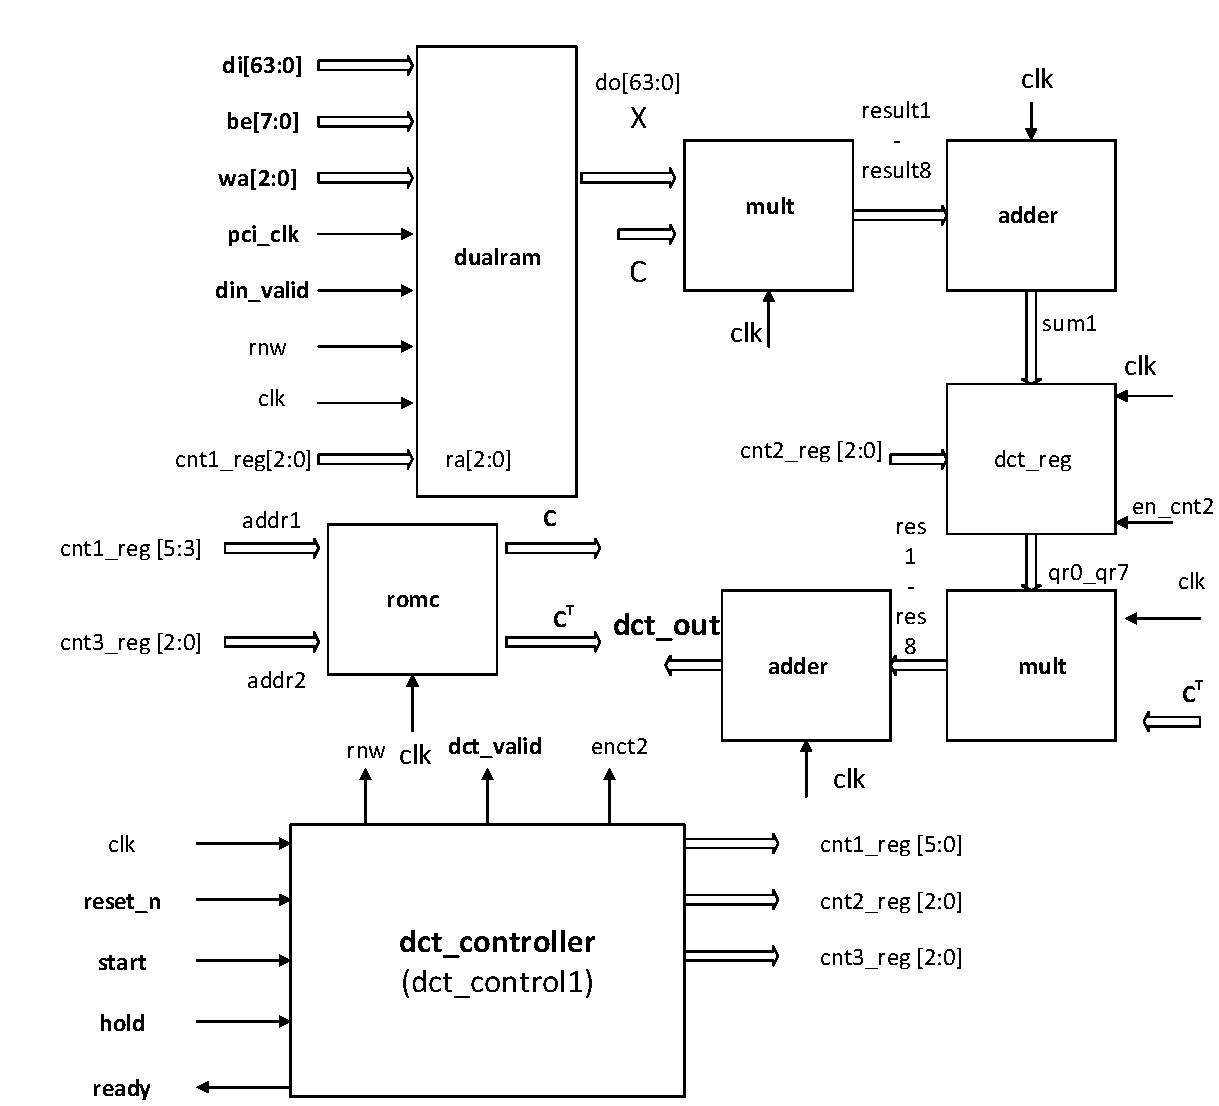
\includegraphics[width=\linewidth]{Figures/System.pdf}
		\caption{Kiến trúc bộ nhân song song} 
		\label{sys}
	\end{figure}
	Từng hàng của khối 8 x 8 được đưa tới đầu vào qua bus dữ liệu, mỗi pixel có 8 bits, $di[7:0]$ là pixel đầu tiên còn $di[63:56]$ là pixel cuối của hàng. $be[7:0]$ gồm 1 byte là tín hiệu enable đầu vào, $be[0]$ chọn $di[7:0]$ và tương tự, $wa[2:0]$ cung cấp địa chỉ hàng của khối ảnh, $wa[0]$ là hàng đầu tiên. $pci_clk$ là xung clock đồng bộ đầu vào, tại sườn lên của xung clock, $di[63:0]$ được ghi vào trong core nhờ tín hiệu $wa[2:0]$. $din\_valid$ lên trạng thái cao nếu $di[63:0]$ hợp lệ.\\
	Quá trình DCT có thể được kiểm soát bởi controller qua tín hiệu $hold$, khi tín hiệu này ở mức thấp thì quá trình diễn ra bình thường. $clk$ là xung đồng hồ của hệ thống, có thể giống với $pci\_clk$. $ready$ chỉ ra rằng DCT core có sẵn sàng hoạt động hay không. Đầu ra DCT dạng bù hai được đưa ra tại $dct[8:0]$ ở sườn lên xung clock. $addr[63:0]$ là địa chỉ các hệ số DCT, $addr[0]$ là hệ số DC, còn lại là hệ số AC. $dct\_valid$ chỉ ra tính hợp lệ của các hệ số DCT và địa chỉ của chúng. Bộ controller có thể reset bất cứ lúc nào nếu tín hiệu $reset\_n$ bằng 0. $Dualram$ chứa bộ nhớ RAM cho hai khối ảnh. Khi một trong hai khối được ghi dữ liệu, quá trình DCT diễn ra qua việc đọc dữ liệu từ khối còn lại một cách đồng thời. Việc ghi dữ liệu vào một khối diễn ra trong 8 chu kỳ $pci\_clk$, trong khi việc đọc dữ liệu của bộ xử lý DCT diễn ra trong 64 $clk$. $cnt1\_reg [2:0]$ tạo ra từ $dct\_controller$, hoạt động như là địa chỉ để lấy nội dung của $dualram$. $rnw$ chọn RAM bank phù hợp. Khi đọc thì RAM sẽ đọc từng cột vì cần thực hiện phép nhân $C*X$, kết quả của phép nhân là $result1 - result8$ được cộng với nhau, kết quả $sum1$ được lưu trong tập thanh ghi $dct\_reg$. Tập thanh ghi này gồm 8 thanh ghi lưu 8 giá trị 11 bits $qr0 - qr7$ là tích $C*X$. Các giá trị này dùng để thực hiện phép nhân $(C*X)*C^T$ trong tám $clk$ tiếp theo. $cnt2\_reg [2:0]$ chọn một trong tám thanh ghi tại một thời điểm. Kết quả của phép nhân này là $res1 - res8$, chúng được cộng với nhau được kết quả là $dct\_out$. Ma trận $C$ và $C^T$ được lưu trong bộ nhớ ROM $romc$, các tín hiệu $cnt1\_reg[5:3]$ và $cnt\_reg[2:0]$ được tạo ra từ controller như là địa chỉ để lấy các hệ số của $C$ và $C_T$ 
	\section{Kết quả và bàn luận}
	Kết quả mô phỏng được thể hiện ở Hình \ref{res}.\\
	\begin{figure}[h]
		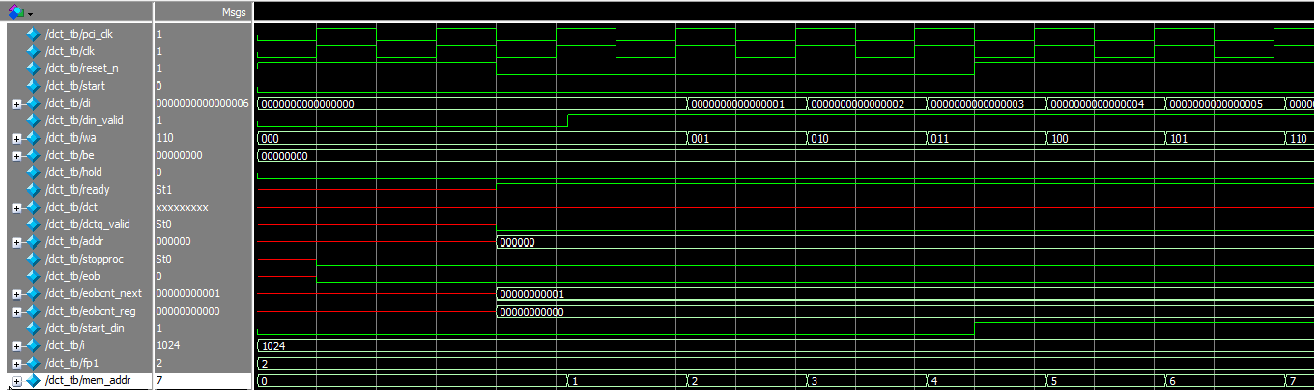
\includegraphics[width=\linewidth]{Figures/result.png}
		\caption{Kết quả mô phòng DCT} 
		\label{res}
	\end{figure}
	Do phần code của bọn em còn chưa chính xác nên chưa đạt được kết quả.
	\section{Kết luận}
	Trong quá trình thực hiện bài tập lớn, chúng em đã có cơ hội tìm hiểu về DCT giúp giảm tải trong quá trình truyền, thực hiện thiết kế từng khối để thực hiện kĩ thuật DCT 64 điểm và thực hiện lập trình Verilog để mô tả hệ thống.
	Qua bài tập lớn chúng em đã học được rất nhiều về việc thiết kế một hệ thống, tuy còn nhiều thiếu sót do thiếu kinh nghiệm nhưng cơ bản chúng em đã hiểu các khâu trong việc phân tích và thiết kế một hệ thống. Đây sẽ là kiến thức nền tảng giúp chúng em trong quá trình học tập, nghiên cứu và phát triển sau này.
	\section{Tài liệu tham khảo}
	\bibliographystyle{IEEEtran}
	\bibliography{mybibfile} 
\end{document}